% Class final report using the Interspeech 2026 Paper Kit format:
% https://www.overleaf.com/latex/templates/interspeech-paper-kit/svqkgcpdbxfg

\documentclass[cameraready]{Interspeech}

\title{Read or Spontaneous? Speech Style Effects on Speaker Verification for L2 English}

\author[affiliation={1}]{Lina}{Na}
\address{$^1$ University of Zurich, Switzerland}
\email{lina.na@uzh.ch}

\keywords{speaker verification, L2 English, speaking style}

\usepackage{booktabs,multirow,tikz}
\usepackage{float}
\usetikzlibrary{positioning, fit, backgrounds, arrows.meta}
\setcounter{topnumber}{3}
\setcounter{bottomnumber}{3}
\setcounter{totalnumber}{5}

\begin{document}
\maketitle

\begin{abstract}
Speaker verification systems decide whether two short utterances come from the same person. In practice, enrollment is often scripted while authentication happens on free speech, yet most benchmarks keep read and spontaneous trials separate. Style mismatch raises equal error rate (EER) on native English; less is known for L2 talkers. We evaluate SpeechBrain x-vector and ECAPA-TDNN checkpoints (VoxCeleb-pretrained, no fine-tuning) on L2-ARCTIC and Svarah under three trial types: Read--Read, Spontaneous--Spontaneous, and Read--Spontaneous. On Svarah, RR gives the lowest EER (x-vector 6.09\%, ECAPA 2.09\%); SS and RS are much worse (up to 28.53\% and 25.09\% for x-vector). ECAPA beats x-vector in every condition. L2-ARCTIC spontaneous data are sparse---one long recording per speaker, split into $\sim$10\,s chunks---so results there are harder to interpret; still, RS raises x-vector EER from 6.25\% to 8.18\%. Code and results: \url{https://github.com/NeoCitran-oss/myFinal}.
\end{abstract}

\section{Introduction}
\label{sec:intro}

Speaker verification asks whether two speech clips belong to the same talker. Current systems encode each utterance with a neural network (x-vector or ECAPA-TDNN) and score cosine similarity between embeddings~\cite{snyder2018xvector,desplanques2020ecapa}. This works well on VoxCeleb-style interview and read speech~\cite{chung2018voxceleb,desplanques2020ecapa}, but real use is messier: someone may enroll by reading a prompt and later speak spontaneously on a call. Read speech is steady and scripted; spontaneous speech has pauses, restarts, and shifting prosody~\cite{kenny2014style}. Cross-style trials increase EER on native data~\cite{tom2010style,park2018style,javali2024style,martinek2025read}, and the gap may grow for L2 speakers who articulate differently when reading than when speaking freely~\cite{zhao2018l2arctic}.

Indian-accented English is common in the wild but rare in verification benchmarks~\cite{javed2023svarah}. L2-ARCTIC offers multi-L1 read speech plus a small spontaneous set~\cite{zhao2018l2arctic}; Svarah pairs read passages with conversational prompts~\cite{javed2023svarah}. Neither has been tested much with modern embeddings under explicit style splits.

We ask whether Martinek \textit{et al.}'s read/spontaneous findings on native RaT data~\cite{martinek2025read} carry over to L2 English. Using the same SpeechBrain checkpoints and a three-condition trial setup, we run x-vector and ECAPA-TDNN on both corpora without fine-tuning. All scripts and indices are on GitHub (\url{https://github.com/NeoCitran-oss/myFinal}).

\section{Related work}
\label{sec:related}

\subsection{Speaker embedding models}

The x-vector model stacks TDNN layers and pools frame statistics into one embedding per utterance~\cite{snyder2018xvector}. ECAPA-TDNN adds channel attention and attentive pooling~\cite{desplanques2020ecapa} and usually beats x-vector on standard benchmarks. We take both from SpeechBrain's VoxCeleb checkpoints~\cite{ravanelli2021speechbrain,chung2018voxceleb}; Figure~\ref{fig:sota} sketches the two pipelines.

\begin{figure}[H]
  \centering
  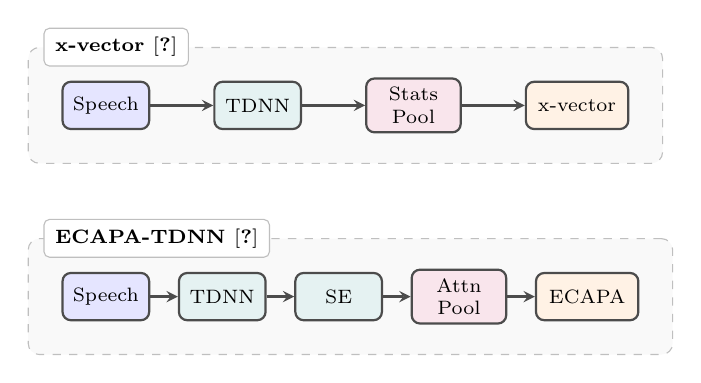
\begin{tikzpicture}[
    font=\scriptsize\rmfamily, 
    >=stealth,
    block/.style={draw=black!70, thick, rounded corners=3pt, minimum height=0.6cm, align=center},
    input/.style={block, fill=blue!10, minimum width=1.1cm},
    layer/.style={block, fill=teal!10, minimum width=1.1cm},
    pool/.style={block, fill=purple!10, minimum width=1.2cm},
    output/.style={block, fill=orange!10, minimum width=1.3cm},
    arrow/.style={->, thick, draw=black!70},
    groupbox/.style={draw=gray!50, fill=gray!5, rounded corners=4pt, dashed, inner sep=12pt}
  ]
    \node[input]  (in1)   {Speech};
    \node[layer, right=0.8cm of in1] (tdnn1) {TDNN};
    \node[pool,  right=0.8cm of tdnn1] (pool1) {Stats\\Pool};
    \node[output, right=0.8cm of pool1] (out1)  {x-vector};
    \draw[arrow] (in1) -- (tdnn1);
    \draw[arrow] (tdnn1) -- (pool1);
    \draw[arrow] (pool1) -- (out1);

    % ==========================================
    \node[input, below=1.8cm of in1] (in2) {Speech};
    \node[layer, right=0.35cm of in2] (tdnn2) {TDNN};
    \node[layer, right=0.35cm of tdnn2] (se) {SE};
    \node[pool,  right=0.35cm of se] (apool) {Attn\\Pool};
    \node[output, right=0.35cm of apool] (out2) {ECAPA};
    \draw[arrow] (in2) -- (tdnn2);
    \draw[arrow] (tdnn2) -- (se);
    \draw[arrow] (se) -- (apool);
    \draw[arrow] (apool) -- (out2);

    % ==========================================
    \begin{scope}[on background layer]
      \node[groupbox, fit=(in1) (out1)] (box1) {};
      \node[groupbox, fit=(in2) (out2)] (box2) {};
    \end{scope}

    \node[above right=-0.25cm and 0.2cm of box1.north west, fill=white, draw=gray!50, rounded corners=2pt, inner xsep=4pt, font=\scriptsize\bfseries] {x-vector~\normalfont\cite{snyder2018xvector}};
    \node[above right=-0.25cm and 0.2cm of box2.north west, fill=white, draw=gray!50, rounded corners=2pt, inner xsep=4pt, font=\scriptsize\bfseries] {ECAPA-TDNN~\normalfont\cite{desplanques2020ecapa}};

  \end{tikzpicture}
  \caption{x-vector and ECAPA-TDNN pipelines (SpeechBrain checkpoints used in this work).}
  \label{fig:sota}
\end{figure}

\subsection{Speaking style and verification}

Style mismatch has been studied for years. Kenny \textit{et al.}~\cite{kenny2014style} and Tom \textit{et al.}~\cite{tom2010style} looked at short segments and conversational vs.\ read trials. Park \textit{et al.}~\cite{park2018style} found large EER jumps when enrollment and test styles differed on sub-2\,s clips, with humans and i-vector systems relying on different cues. Javali \textit{et al.}~\cite{javali2024style} reported similar drops for deep models on read vs.\ spontaneous speech. Hughes \textit{et al.}~\cite{hughes2025voice} showed that regional accent also shifts both human and automatic scores.

Martinek \textit{et al.}~\cite{martinek2025read} are closest to our setup. On the Read-and-Tell (RaT) corpus they compared matched read, matched spontaneous, and mixed enrollment--test pairs with SpeechBrain and Resemblyzer. Uniform styles gave near-zero EER; mixing read and spontaneous pushed error up (e.g.\ 11.57\% for Resemblyzer, 23--33\% for spoof-aware models). They did not test L2 or Indian-accented English. We reuse their RR/SS/RS logic and the same SpeechBrain models on L2-ARCTIC and Svarah.

\subsection{L2 and accented English corpora}

L2-ARCTIC~\cite{zhao2018l2arctic} has read English from 24 non-native speakers (six L1 groups) and suitcase spontaneous descriptions from 22 of them. Svarah~\cite{javed2023svarah} has 9.6\,h of Indian-accented English with both read passages and conversational service prompts. Both are popular for ASR; style-conditioned verification trials on L2 talkers are still scarce next to native work~\cite{martinek2025read,park2018style}.

\section{Motivation}
\label{sec:pitfalls}

Three practical issues drove this evaluation. First, VoxCeleb-trained models are tuned on mostly native interview speech~\cite{chung2018voxceleb,desplanques2020ecapa}; L2 spontaneous clips are a harder, out-of-domain test. Second, papers often publish one corpus-level EER without saying whether enrollment and test were read or spontaneous---a system can look fine on RR and fail on RS~\cite{tom2010style,martinek2025read}. Third, spontaneous--spontaneous trials need multiple spontaneous segments per speaker; L2-ARCTIC only has one long suitcase recording each, so we had to chunk it~\cite{zhao2018l2arctic}, which limits how much we can trust SS numbers.

\section{Method}
\label{sec:method}

We follow a standard text-independent setup. One enrollment utterance in style~$A$ gives embedding $\bar{e}$; one test utterance in style~$B$ gives $e_t$; the score is $\cos(\bar{e}, e_t)$. Target trials use the same speaker; impostor trials swap in another speaker's enrollment (same style~$A$). EER is the threshold where false accept and false reject rates match~\cite{snyder2018xvector}.

We test three conditions for each corpus and model:
\begin{itemize}
  \item \textbf{RR} --- read enrollment, read test;
  \item \textbf{SS} --- spontaneous enrollment, spontaneous test;
  \item \textbf{RS} --- read enrollment, spontaneous test (cross-style).
\end{itemize}

Following~\cite{martinek2025read,park2018style,javali2024style}, we expect RS (and often SS) to give higher EER than RR, with ECAPA doing better than x-vector~\cite{desplanques2020ecapa}.

\subsection{Models}

We use SpeechBrain checkpoints \texttt{spkrec-xvect-voxceleb} and \texttt{spkrec-ecapa-voxceleb}~\cite{ravanelli2021speechbrain} with no fine-tuning. Audio is mono at \SI{16}{\kilo\hertz}. We skip score normalization so results reflect raw embedding similarity on L2 data.

Figure~\ref{fig:protocol} illustrates the trial flow. Table~\ref{tab:protocol} lists hyperparameters.

\begin{figure}[H]
  \centering
  \fbox{\parbox{0.92\linewidth}{\centering\vspace{0.8em}
  \small
  \textbf{Step 1:} Select enrollment utterance(s) in style A \\
  $\rightarrow$ extract embedding(s) $\rightarrow$ $\bar{e}$ \\
  \textbf{Step 2:} Select test utterance in style B $\rightarrow$ $e_t$ \\
  \textbf{Step 3:} score $= \cos(\bar{e}, e_t)$ \\
  Target trial: same speaker; impostor trial: different speaker \\
  \vspace{0.8em}}}
  \caption{Trial construction: enroll in style~$A$, test in style~$B$. RR and SS keep $A{=}B$; RS uses read then spontaneous.}
  \label{fig:protocol}
\end{figure}


\begin{table}[H]
  \caption{Fixed settings for all runs (five impostors per target trial).}
  \label{tab:protocol}
  \centering
  \begin{tabular}{ll}
    \toprule
    Setting & Value \\
    \midrule
    Sample rate & \SI{16}{\kilo\hertz} \\
    Enrollment utterances & 1 \\
    Impostors per target trial & 5 \\
    Scoring & Cosine similarity \\
    Metric & Equal error rate (EER) \\
    Random seed & 42 \\
    \bottomrule
  \end{tabular}
\end{table}

\section{Datasets}
\label{sec:datasets}

\subsection{L2-ARCTIC}

L2-ARCTIC~\cite{zhao2018l2arctic} has 24 L2 speakers (four per L1) and suitcase spontaneous speech from 22 of them. We use the KoelLabs HuggingFace split~\cite{koellabs2024l2arctic}: 3{,}599 read utterances and 22 spontaneous recordings.

Each speaker has only one spontaneous recording, so we cut it into $\sim$\SI{10}{\second} chunks (162 segments total, $\sim$7.4 per speaker) to run SS trials. Chunks from the same session are correlated, which is a real limitation of this corpus for spontaneous verification.

\subsection{Svarah}

Svarah~\cite{javed2023svarah} covers 117 Indian-accented speakers with read passages and conversational prompts (passport queries, grocery orders, etc.). The public \texttt{test} split has no style label, so we tagged utterances from transcript cues: questions and short service replies $\rightarrow$ spontaneous; narrative passages $\rightarrow$ read. After keeping speakers with both tags, 110 remain. Official labels would be preferable if NPTEL releases them.

\subsection{Download}

Data come through HuggingFace (\texttt{download.py}; gated sets need \texttt{hf auth login}). Setup and index layout are documented in the repository README at \url{https://github.com/NeoCitran-oss/myFinal/blob/main/README.md}.

\section{Hypotheses}
\label{sec:hypotheses}

\begin{itemize}
  \item \textbf{H1:} RS and SS give higher EER than RR on L2 data~\cite{martinek2025read,park2018style,javali2024style}.
  \item \textbf{H2:} ECAPA beats x-vector in all conditions~\cite{desplanques2020ecapa}.
  \item \textbf{H3:} Style effects show up more clearly on Svarah than on L2-ARCTIC (more spontaneous material per speaker).
\end{itemize}

\section{Experiments}
\label{sec:experiments}

\subsection{Pipeline}

The repo has five Python modules (\url{https://github.com/NeoCitran-oss/myFinal}): \texttt{config.py}, \texttt{core.py}, \texttt{download.py}, \texttt{run\_eval.py}, and \texttt{run\_ablation\_enroll.py}. Each wav file gets a speaker ID and style tag in a JSON index. Trials are built with seed 42; embeddings use \texttt{EncoderClassifier.encode\_batch}; EER is computed per corpus, model, and condition.

\subsection{Setup}

Runs used a Linux server with \texttt{--device auto} (ablation fell back to CPU when CUDA failed). Checkpoints sit in \texttt{hf\_cache/}. No tuning---only off-the-shelf weights.

\subsection{Enrollment ablation}

On Svarah RR we also tried two read enrollment utterances instead of one, averaging their embeddings~\cite{snyder2018xvector}. Results are in Section~\ref{sec:results}.

\subsection{Trial counts}

Table~\ref{tab:trialcounts} summarizes speakers and trials. L2-ARCTIC RR includes all 24 read speakers; SS and RS include 22 speakers with spontaneous material. Svarah RR and RS use 110 speakers; SS uses 109 speakers with at least two spontaneous segments.

\begin{table}[H]
  \caption{Number of target speakers and total verification trials (target + impostor) per corpus and condition for the x-vector system (trial counts are identical across models).}
  \label{tab:trialcounts}
  \centering
  \begin{tabular}{lcccc}
    \toprule
    Corpus & Condition & Target spk. & Trials \\
    \midrule
    \multirow{3}{*}{L2-ARCTIC} & RR & 24 & 144 \\
     & SS & 22 & 132 \\
     & RS & 22 & 132 \\
    \midrule
    \multirow{3}{*}{Svarah} & RR & 110 & 660 \\
     & SS & 109 & 654 \\
     & RS & 110 & 660 \\
    \bottomrule
  \end{tabular}
\end{table}

\section{Results}
\label{sec:results}

Table~\ref{tab:results} lists EER by corpus, model, and condition; Figure~\ref{fig:eer_compare} plots Svarah, where the style gap is largest.

\begin{table}[H]
  \caption{Equal error rate (EER, \%) on L2-ARCTIC and Svarah for x-vector and ECAPA-TDNN under three enrollment--test style conditions. RR: read--read; SS: spontaneous--spontaneous; RS: read enrollment with spontaneous test. L2-ARCTIC spontaneous trials use $\sim$\SI{10}{\second} chunks from single suitcase recordings per speaker.}
  \label{tab:results}
  \centering
  \begin{tabular}{llccc}
    \toprule
    Corpus & Model & RR & SS & RS \\
    \midrule
    \multirow{2}{*}{L2-ARCTIC} & x-vector & 6.25 & 2.27 & 8.18 \\
     & ECAPA-TDNN & 0.00 & 0.45 & 0.00 \\
    \midrule
    \multirow{2}{*}{Svarah} & x-vector & 6.09 & 28.53 & 25.09 \\
     & ECAPA-TDNN & 2.09 & 12.57 & 10.55 \\
    \bottomrule
  \end{tabular}
\end{table}

\begin{figure}[H]
  \centering
  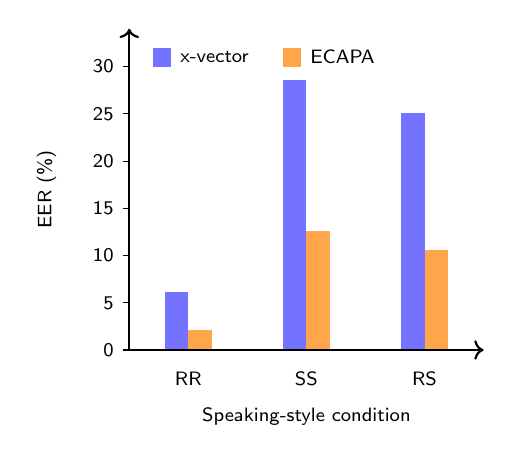
\begin{tikzpicture}[font=\scriptsize\sffamily, x=1.5cm, y=0.12cm]
    \def\bw{0.2} % bar width

    % x-vector bars (Left bar in each group)
    \fill[blue!55] (1-\bw, 0) rectangle ++(\bw, 6.09);
    \fill[blue!55] (2-\bw, 0) rectangle ++(\bw, 28.53);
    \fill[blue!55] (3-\bw, 0) rectangle ++(\bw, 25.09);

    % ECAPA bars (Right bar in each group)
    \fill[orange!70] (1, 0) rectangle ++(\bw, 2.09);
    \fill[orange!70] (2, 0) rectangle ++(\bw, 12.57);
    \fill[orange!70] (3, 0) rectangle ++(\bw, 10.55);

    % Axes
    \draw[->, thick] (0.5, 0) -- (3.5, 0);
    \draw[->, thick] (0.5, 0) -- (0.5, 34);

    % Y-axis ticks
    \foreach \y in {0, 5, 10, 15, 20, 25, 30} {
      \draw (0.5, \y) -- (0.45, \y) node[left] {\y};
    }

    % X-axis labels
    \node at (1, -3) {RR};
    \node at (2, -3) {SS};
    \node at (3, -3) {RS};
    \node at (2, -7) {Speaking-style condition};

    % Y-axis label
    \node[rotate=90] at (-0.2, 17) {EER (\%)};

    % Legend
    \fill[blue!55] (0.7, 30) rectangle ++(0.15, 2);
    \node[right] at (0.85, 31) {x-vector};
    \fill[orange!70] (1.8, 30) rectangle ++(0.15, 2);
    \node[right] at (1.95, 31) {ECAPA};

  \end{tikzpicture}
  \caption{Svarah EER (\%) by condition. RR is easiest; SS and RS hurt x-vector most.}
  \label{fig:eer_compare}
\end{figure}

\subsection{Svarah}

Svarah matches the pattern Martinek \textit{et al.}~\cite{martinek2025read} saw on native RaT: RR is easiest (x-vector 6.09\%, ECAPA 2.09\%), SS jumps to 28.53\% / 12.57\%, and RS stays high at 25.09\% / 10.55\%. Service-style spontaneous prompts in Svarah~\cite{javed2023svarah} are short and variable, which likely hurts embeddings trained on cleaner speech. Our RS numbers are worse than Martinek's mixed-speech EER on RaT with similar SpeechBrain models, so L2 accent may add to the style penalty.

ECAPA wins in every cell, by up to 16 points on SS. For Indian-accented L2 use, it is the better off-the-shelf pick here, though RS above 10\% is still risky without adaptation.

\subsection{L2-ARCTIC}

ECAPA is near zero on all conditions (0.00--0.45\%), probably because the read studio set is small and easy for a strong VoxCeleb model. x-vector is noisier: RS (8.18\%) sits above RR (6.25\%), as H1 predicts, but SS (2.27\%) is oddly \emph{below} RR. With only 22 speakers and chunked suitcase audio, SS trials share a lot of session-level correlation---we would not read much into that SS number.

\subsection{Cross-corpus}

Svarah shows a clearer read-vs-spontaneous split; L2-ARCTIC is still useful for multi-L1 read speech but weak for spontaneous work without more recordings~\cite{zhao2018l2arctic}. How you build trials matters as much as which model you pick.

\subsection{Hypotheses}

H1 holds on Svarah (RR $<$ RS $\approx$ SS) but only partly on L2-ARCTIC. H2 holds everywhere (ECAPA $<$ x-vector). H3 holds: Svarah has wider EER spread across conditions.

\subsection{Enrollment ablation}

Two enrollment utterances on Svarah RR lower EER (x-vector 6.09\% $\rightarrow$ 3.85\%; ECAPA 2.09\% $\rightarrow$ 1.38\%), even when read style is matched.

\begin{table}[H]
  \caption{Ablation on Svarah Read--Read: EER (\%) vs.\ number of enrollment utterances.}
  \label{tab:ablation}
  \centering
  \begin{tabular}{lcc}
    \toprule
    Model & 1 enroll utt. & 2 enroll utts. \\
    \midrule
    x-vector & 6.09 & 3.85 \\
    ECAPA-TDNN & 2.09 & 1.38 \\
    \bottomrule
  \end{tabular}
\end{table}

\section{Conclusion}
\label{sec:conclusion}

We ran x-vector and ECAPA-TDNN on L2-ARCTIC and Svarah with matched and cross-style trials, extending Martinek \textit{et al.}'s native RaT study~\cite{martinek2025read} to L2 English. Svarah shows the same ranking as RaT---RR best, SS and RS much worse, ECAPA ahead of x-vector~\cite{desplanques2020ecapa}. L2-ARCTIC only weakly supports H1 because spontaneous data are thin and ECAPA already saturates.

Voice login on L2 users should be evaluated by speaking style, not read prompts alone~\cite{javed2023svarah,zhao2018l2arctic}. Next steps: more spontaneous sessions per speaker, fine-tuning on multi-style L2 data, official Svarah style tags, score normalization, and per-L1 breakdowns on L2-ARCTIC. Code: \url{https://github.com/NeoCitran-oss/myFinal}.


\section{Generative AI Use Disclosure}
Generative AI assisted with code and LaTeX formatting; I checked all text and take responsibility for the report.

\bibliographystyle{IEEEtran}
\bibliography{references}

\end{document}
